%----------
\chapter{Fundamental approach}
	Object-relation Mapping can be done in many ways. First, of course, one can implement
	the whole code by hand. As already mentioned, this is not the scope of this thesis
	and is therefore not a possible solution. Second, we have a mechanism to
	automate the coding part. In this thesis, we try to find a good solution to
	generate the code. Another approach would be to supply a set of generic
	classes, which is not our aim, either.
	
	To generate as much code as possible, we need to have information about
	the database structure as well as about the domain model and how
	to map these two. This can be quite a lot the programmer needs to
	know but usually should not be a problem. The intend of \textit{STORM} is
	to provide a programmer a solution, which allows him to specify all these
	information in a, for a programmer, natural way.
	
	The following sections describe 3 possible ways to implement such a tool
	as \textit{STORM}. The pros and cons are mentioned. There is no doubt that
	there exist more possibilities but we hope to give a reasonable overview
	with the following selection.
	
	\section{XML Schema}
		\begin{figure}[htb]
			\begin{center}
				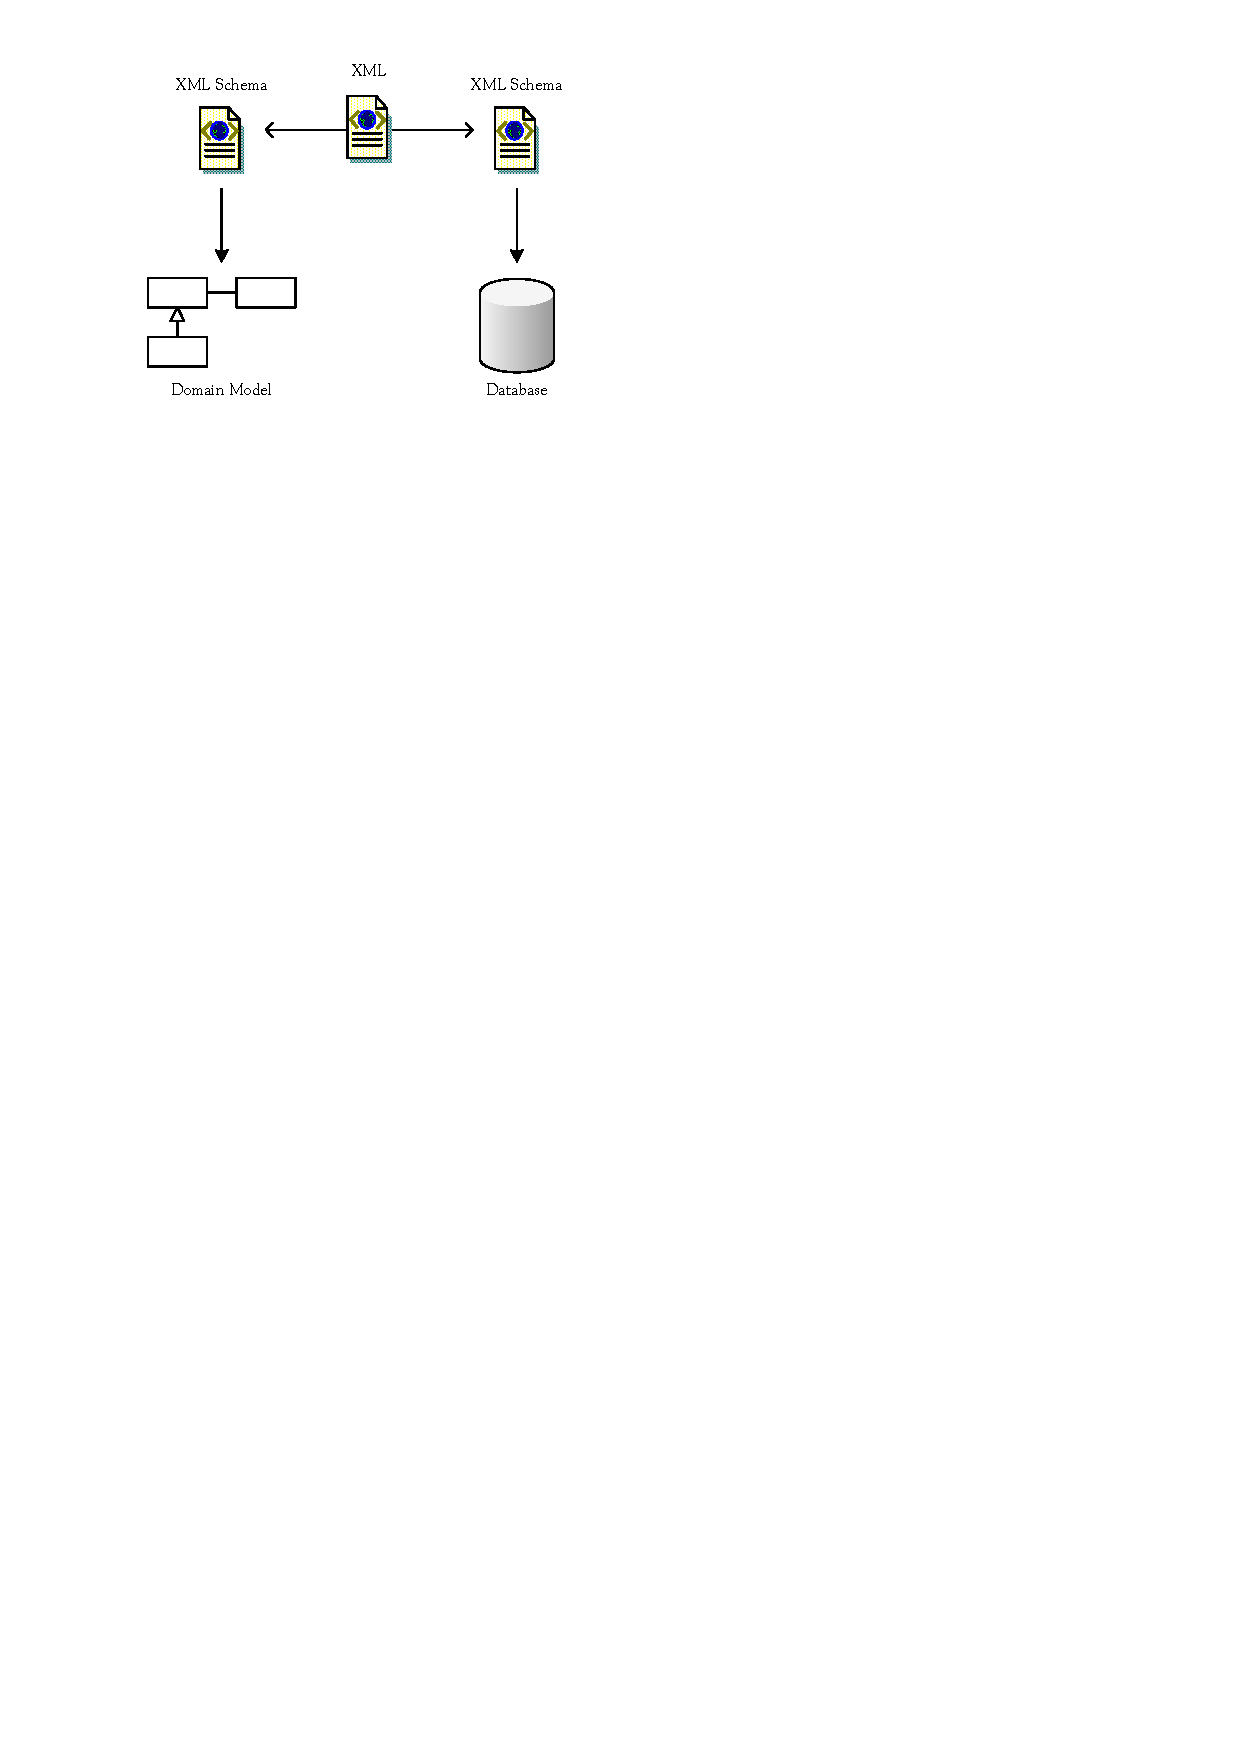
\includegraphics{./files/inc/figures/caseStudyXmlSchema}
				\caption{\label{fig:caseStudyXmlSchema} Mapping description with XML Schema}
			\end{center}
		\end{figure}
		Figure \ref{fig:caseStudyXmlSchema} shows a first possible mechanism to describe
		the information needed to generate mapping code. On the right, an XML Schema file
		is used to reflect the database structure. A sample of such a file is shown in 
		Listing \ref{lst:xsdDbConfig}. This is probably not the most sophisticated
		XML schema possible but nevertheless it is possible to describe a database structure
		with such a file. We implemented a XML schema parser which read the content of
		this file and used it as input for a CodeSmith template.
		
		The main problem with this approach is the XML schema language. It is not possible
		to describe all information needed to generate the mapping code in a schema file.
		This limitation results in the fact that another XML schema file is needed to describe
		the domain model structure (as shown on the left in Figure \ref{fig:caseStudyXmlSchema}).
		Additionally an XML file is needed to specify the mapping between the two schemes. For
		example, this XML file would include a tag describing which database table
		matches to which class in the domain model.
		
		There are a few drawbacks with this solution. One of those is that an XML schema
		is not a natural way a programmer would describe a database structure nor a 
		domain model. Another drawback is its implementation. The schema description must 
		undergo certain restrictions for consistency. A programmer therefore has to adopt
		and respect this restriction when writing a schema file. The implementation
		itself is not easy as well, because a mapping strategy needs to be defined.
		To define such a strategy which allows to specify every possible mapping is not
		an easy task.
		
		On the other hand, there are benefits which makes this approach worth looking
		at. XML schema and XML are well defined and standardised. This makes it 
		possible to delegate the task of writing the XML files to a tool such as
		a database design tool. The only thing which cannot be automated is the 
		XML file describing the mapping.
	
	\begin{lstlisting}[float,language=XML,caption=XML schema describes database structure,label=lst:xsdDbConfig]
<?xml version="1.0" encoding="utf-8" ?>
<xs:schema id="BusinessObjects1" 
		targetNamespace="http://tempuri.org/BusinessObjects1.xsd"
	elementFormDefault="qualified" 
			xmlns="http://tempuri.org/BusinessObjects1.xsd" 
			xmlns:xs="http://www.w3.org/2001/XMLSchema">
	<xs:group name="classes">
		<xs:sequence>
			<xs:element name="Person" type="PersonType" />
			<xs:element name="Address" type="AddressType" />
		</xs:sequence>
	</xs:group>
	<xs:complexType name="AddressType">
		<xs:sequence>
			<xs:element name="Person" type="PersonType" />
			<xs:element name="Street">
				<xs:simpleType>
					<xs:restriction base="xs:string">
					</xs:restriction>
				</xs:simpleType>
			</xs:element>
			<xs:element name="City">
				<xs:simpleType>
					<xs:restriction base="xs:string">
					</xs:restriction>
				</xs:simpleType>
			</xs:element>
	</xs:complexType>
</xs:schema>
	\end{lstlisting}
		
	\section{Abstract Class with Attributes}
		A second approach to describe the mapping is to write an abstract class
		with custom attributes. A code snippet of such a class is shown in Listing
		\ref{lst:abstractClass}. This class file is compiled at runtime and the custom
		attributes can be read using reflection from the resulting dll. With these attributes,
		all needed information can be retrieved.
		
		The main advantage of this is that a programmer can define everything in a single file
		rather than multiple files. Furthermore it is a more natural way for programmers because
		they are used to write classes.
		
		One could say that a drawback of attributes is that they cannot be changed at runtime.
		This is true but also, it is not required. Every information given in this 
		abstract class is static within the scope of an application. As mentioned above,
		C\# reflection mechanism is used to read the settings. This is constricted to
		the process of generating code. The generated code does not make use of reflection. This
		would be possible but would result in a poorer performance.
		
		From our point of view, this approach is the most feasible.
	
	
	\begin{lstlisting}[float,language={[Sharp]C},caption=Abstract class with custom attributes,label=lst:abstractClass]
[Table("Addresses", true),
VersionField("chTimeStamp", typeof(Timestamp))]
public abstract class Address : DomainObject
{
	[Column("AddressID"),
		PrimaryKey]
	public abstract int AddressId {get; set;}

	[Column("City")]
	public abstract string City {get; set;}

	[Column("Street")]
	public abstract string Street {get; set;}
}
	\end{lstlisting}
	
	\section{Extended C\# Compiler}
		This is the most advanced approach and would give the highest possible flexibility. The
		basic idea is to take an existing C\# compiler and extend it to work with custom defined
		keywords. With this new introduced keywords, the mapping information could be given in a
		well defined, familiar manner.
		
		Due to the limited time for this thesis, we do not follow this approach in more detail, 
		although it would be very interesting and promising. A possible solution could be to
		use a compiler generation tool such as Coco/R \cite{Coco/R}.
			